\documentclass{acm_proc_article-sp}
\usepackage{graphicx}
\usepackage{algorithm}

\usepackage{algpseudocode}
\usepackage{amsmath}
\usepackage{graphics}
\usepackage{epsfig}

\begin{document}
\title{Source code analyzing with parallel programming technique}
\subtitle{NCTU Parallel programming 2015 Fall Final project}

\numberofauthors{3}
\author{
\alignauthor
Tseng Yi\\
       \affaddr{0356063}\\
       \affaddr{National Chiao Tung University}\\
\alignauthor
Wang Hsu Chien\\
       \affaddr{0356136}\\
       \affaddr{National Chiao Tung University}\\
\alignauthor
Chiang Sheng Yi\\
       \affaddr{0356549}\\
       \affaddr{National Chiao Tung University}\\
}

\date{11 3 2015}

\maketitle
\begin{abstract}
       This project shows that the performance improved while using multithread technique
       to analyzing million-line level source code like linux. Include line count, statement counting
       and function call recording.
\end{abstract}

\keywords{Parallel programming, pthread, code analyzing}

\section{Introduction}
\subsection{Background}
       Source code optimizing is one of key technique of compiler. 
       It's important to optimize source code for better performance, 
       less memory usage\ldots as so on. It's not enough by optimizing 
       source code by using compiler. We need to change the source 
       code and find the better way to implement our program. 
\subsection{Importance}
	By using simple analyzing program, we can find which statement we 
	use a lot, how many local variable we create, or how many useless 
	function we write. With those analyze data, developers can improve performance,
	decrease memory usage by reduce function calls or memory allocate.
\subsection{Motivation}
	However, it cost too much times to analyze source code while there
	exist a lots lines in our code, for example Linux kernel.
	We introduce a source code analyzer for million-line source code
	by using multi-thread technique, and compare the performance with 
	single thread analyzer.


\section{The problem}
\subsection{Performance of analyzing source code}
	There are a lot of ways to analyzing code, for example, calculate
	line number or statement number to let developer know the 
	volume of one program. We found that, there are many things that
	cause low performance for one program, such as increasing number 
	of recursive function call, or use less memory allocate.
	In this project, we want to calculate number of function calls and 
	number of \textbf{branch} statement like \textbf{if, switch, while, for}\ldots
	For single thread analyzer, if there are \textit{N} lines in one source file, 
	and there exist \textit{W} files in the project, assume that there only one 
	statement in one line, the time complexity is \textit{O(NW)}. Notice that
	NW is equals to total lines of the project.
	Next we need to figure out how to parse one line. The simplest way 
	to know which statement in specific line is using regular expression 
	and searching keywords, the time complexity of text searching is 
	\textit{O(TP)} where \textit{T} is length of text(line) and \textit{P} is length
	of pattern. Now we notice that each line, or file can be independent 
	if we only need to calculate specific statements or function calls, so
	we might improve performance by using parallel programming technique.

\section{Approach}
\subsection{Architecture of analyzer}
	Figure 1 shows the architecture of our program, there exist one dispatcher 
	and several analyzers, each analyzer will use one thread. Initially, the 
	dispatcher will scan all the project and create an index of all files, then
	it will generate multiple thread for analyzer. After generated thread, 
	dispatcher will send \textbf{block}s into analyzers.

\begin{figure}
	\centering
	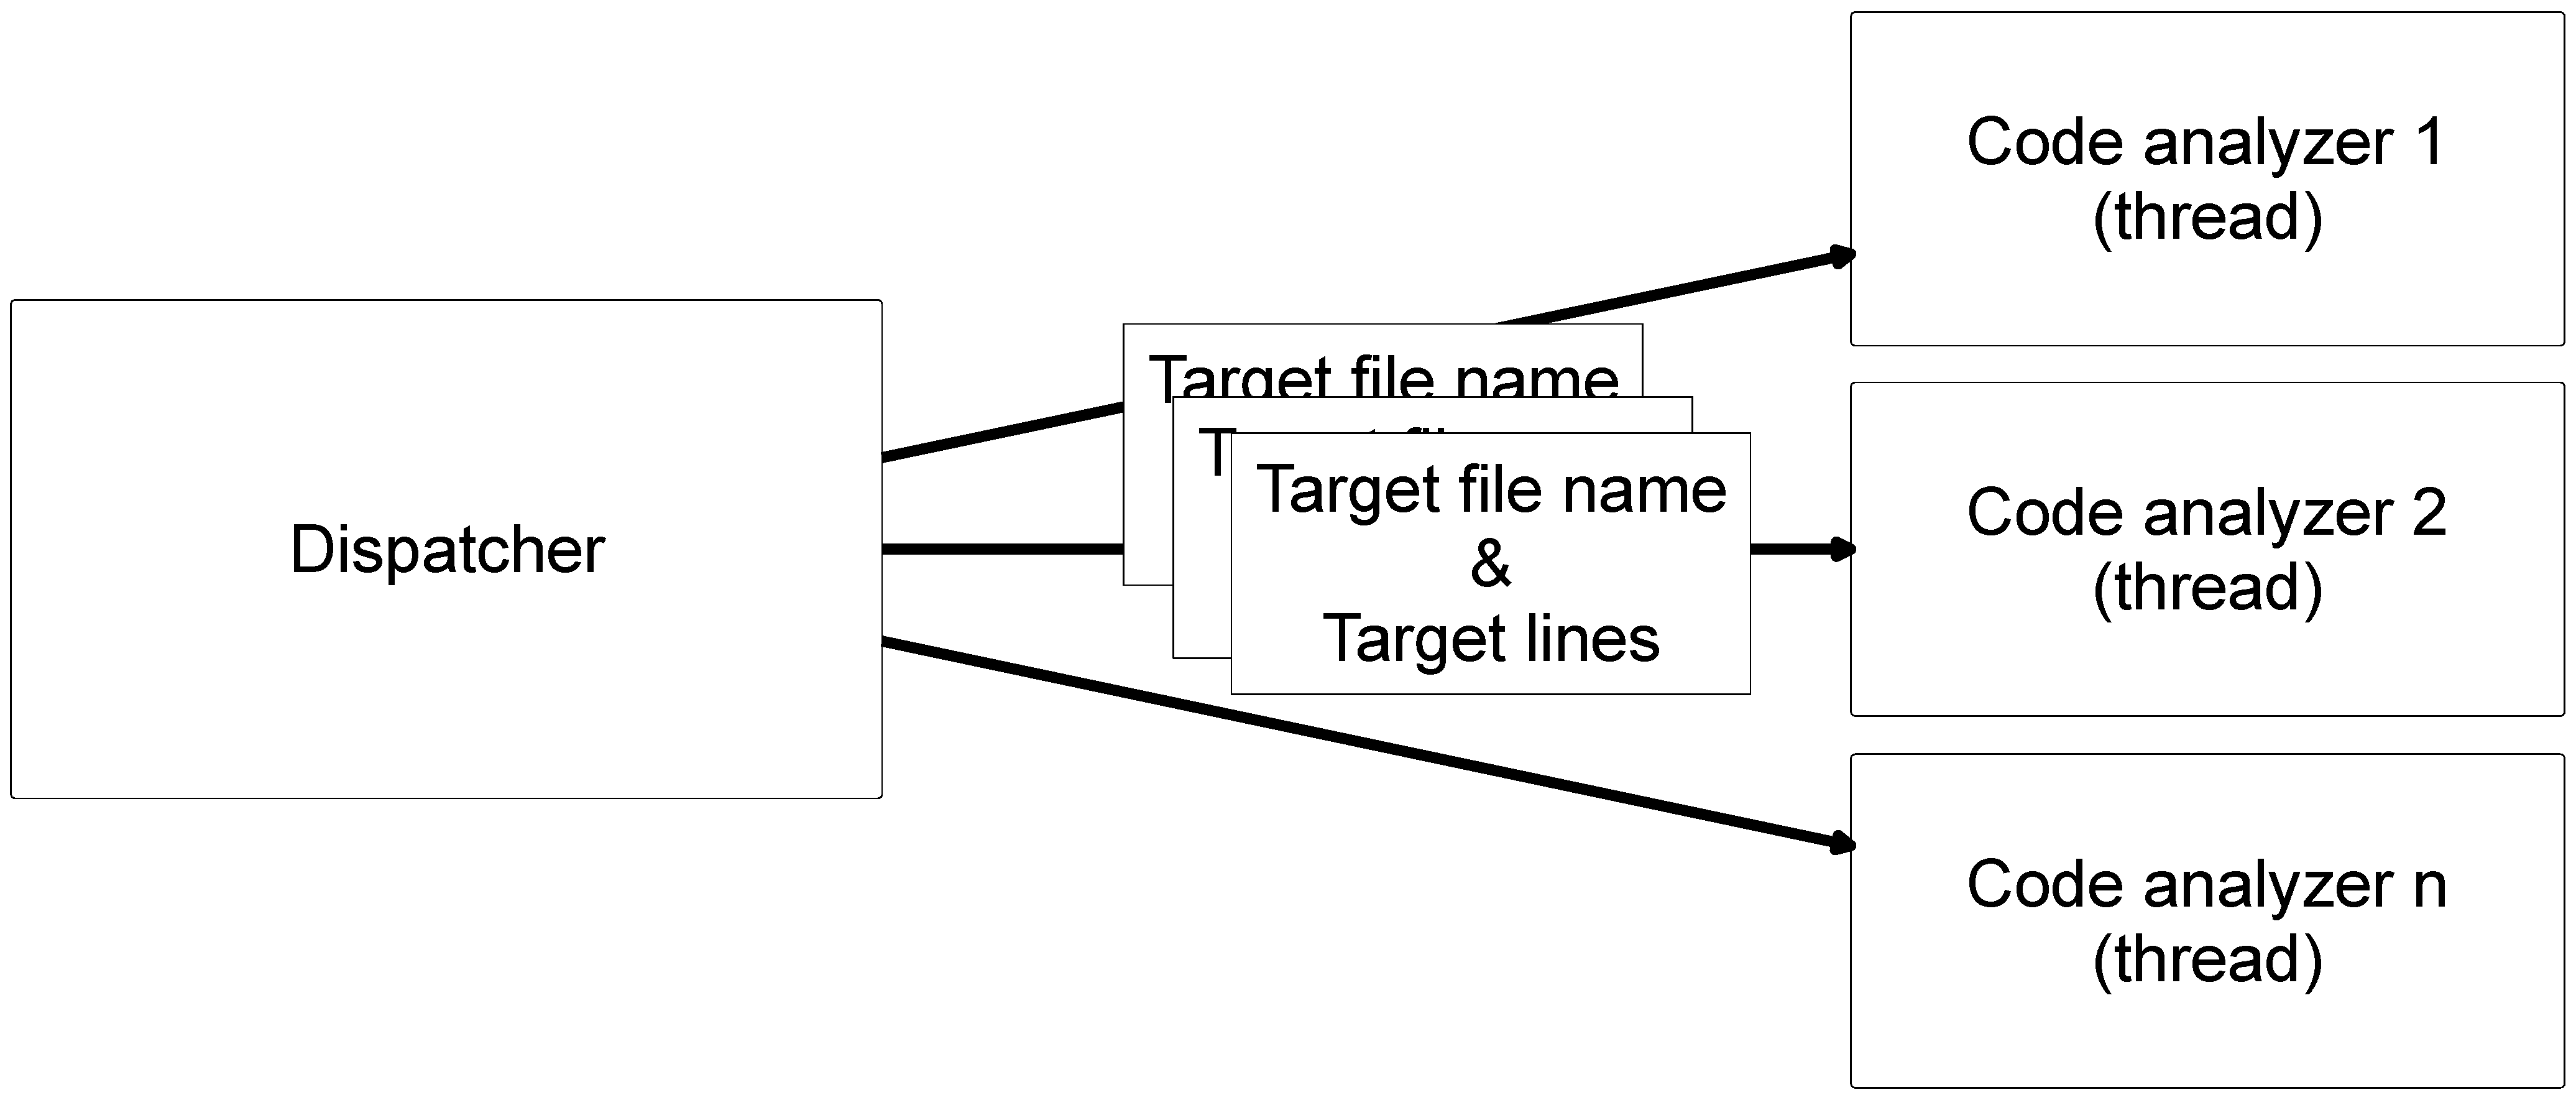
\epsfig{width=8cm, file=architecture.eps}
	\caption{Architecture}
\end{figure}


\subsection{Components}
\subsubsection{Dispatcher}
	The dispatcher will use list of source code files and convert all files into
	\textbf{block}s. Figure 2 shows that many source file split into many blocks
	, and dispatch into many analyzers. To find the ``cut'' point, first we need to 
	get total line of all source code, and divide it by number of thread(analyzer)
	that we need to use.
\begin{figure}
	\centering
	\epsfig{width=8cm, file=code_slice.eps}
	\caption{Slice source file into multiple blocks}
\end{figure}
\subsubsection{Code analyzer}
	Code analyzer will search specific pattern or syntax of one line, and record 
	it to it memory scope. There contains several functions in the analyzer:
	\begin{enumerate}
		\item Search \textbf{branch} statement like if, switch...
		\item Record function call
		\item Record number of statements(split by semicolumn)
	\end{enumerate}
	
\subsection{Workflow}
	Figure 3 shows the work flow of our program, there contains four part:
	\begin{enumerate}
		\item Scan: scan all file, recording number of lines of each file
		\item Dispatch: generate thread and send code blocks to it
		\item Analyze: analyze source code
		\item Merge: merge the result from analyzers
	\end{enumerate}

\begin{figure}
	\centering
	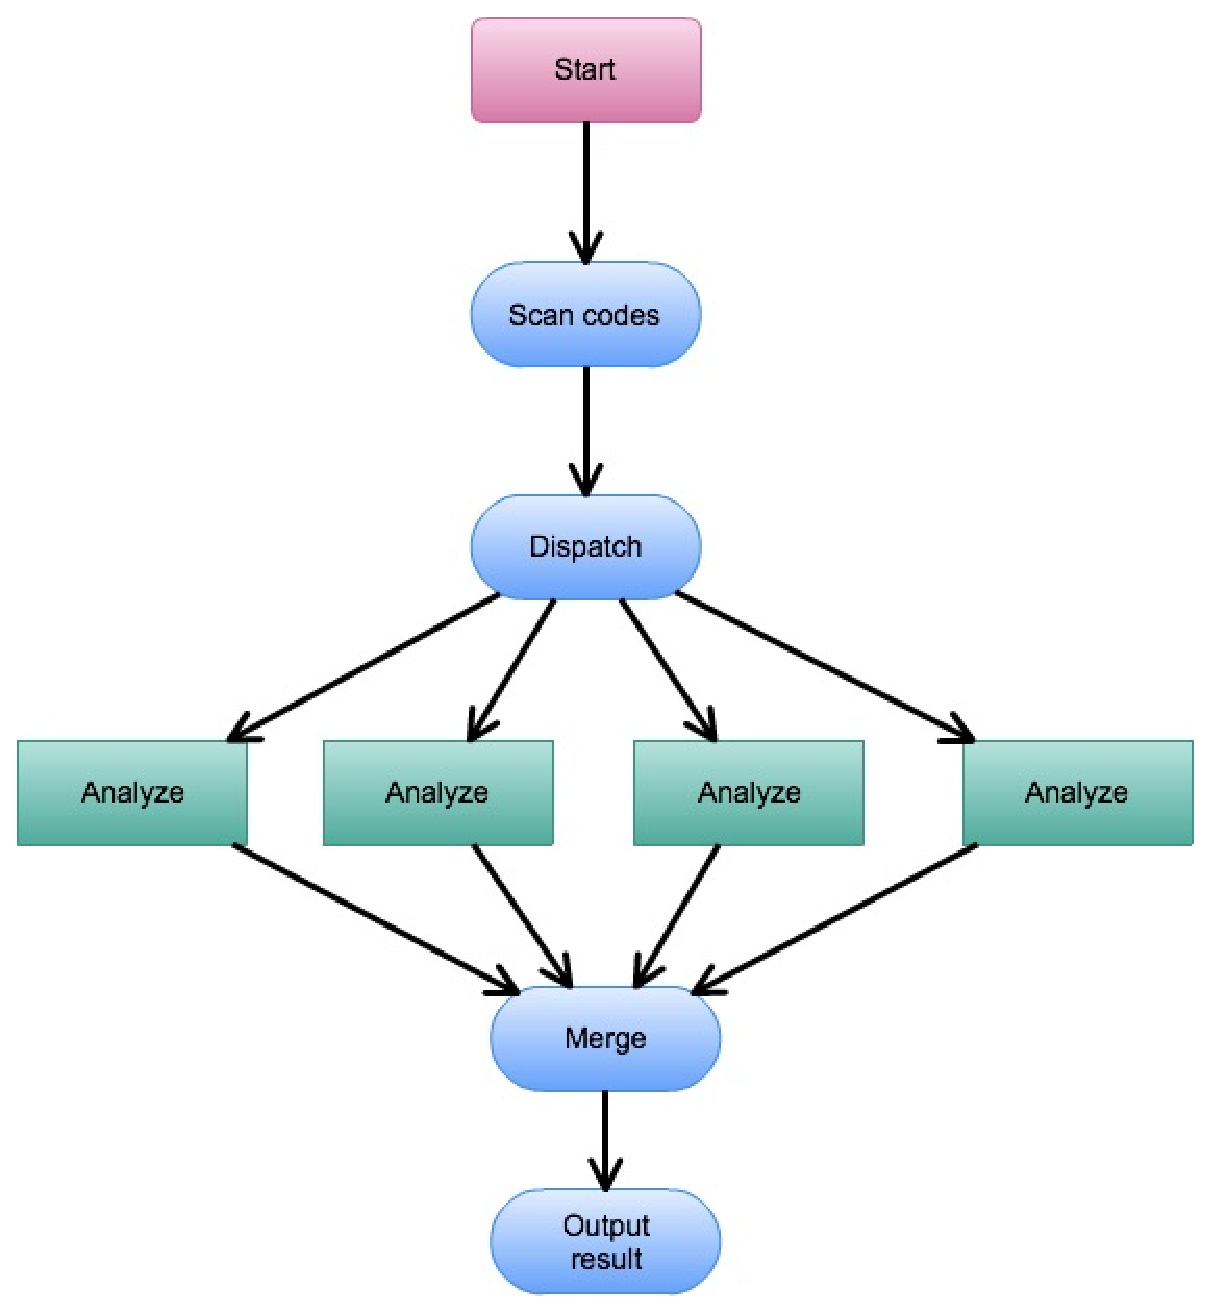
\epsfig{width=8cm, file=flow_chart.eps}
	\caption{Program workflow}
\end{figure}

\section{Language selection}
	In this project, we will use C++ with OpenMP multi-threading library.
	OpenMP (Open Multi-Processing) is an application programming interface 
	(API) that supports multi-platform shared memory multiprocessing 
	programming in C, C++, and Fortran. OpenMP is already built-in library in 
	C/C++ which is the language we are familiar with. OpenMP can be used on 
	various accelerators such as GPGPU. Original code statements do not 
	need to be modified when parallelized with OpenMP, this reduces the chance 
	of inadvertently introducing bugs. OpenMP does not need to deal with message 
	passing as MPI does. For the above reasons, OpenMP is a good choice for 
	out project.
	
\section{Proposed Solution}
\subsection{Single thread/process solution}
	To simply analyze code, we use \textit{regular expression}[4] to convert source
	code into \textbf{tokens}, and use these tokens to get information of each line
	of source code. For example, follow expression shows the regular expression of function call: 
	\begin{displaymath}
		[a-zA-Z_][a-zA-Z0-9_]+(.*);
	\end{displaymath}
	After convert code into tokens, we can record the number of each tokens. Also
	record function or variable names.
	Follow code is the basic algorithm of code analyzing.
	\begin{algorithm}[h]
		\caption{Single thread code analyze}
		\begin{algorithmic}[1]
			\Require
				$get_token(x)$: parse code and get token list;
				$num_lines$: total lines of source code;
				$s$: source code file pointer;
				$next\_line(s)$: get next line from source code;
			\State initial $current_line=0$ and $token\_table is empty$;
			\Repeat
				\State $line$ = $next\_line(s)$
				\State $token\_list$ = $get\_token(line)$
				\For{each $token \in $token\_list}
					\State $token\_table[$token]++
				\EndFor
				\State $current\_line$ = $current\_line + 1$
			\Until{$current\_line \ne num\_lines$}
		\end{algorithmic}
	\end{algorithm}

\section{Related work}

	\textbf{quantifiedcode}[3] provide online python code analyzer, it can let developer 
	know how to improve his/her code by giving some suggestions.
	nowadays, in multiple research, we can find that code analysis can be used to 
	detect malware software, this kind of static analysis take less resources and time. 
	It’s much easier than dynamic analysis method.



\section{References}
[1] OpenMP: 2015. http://openmp.org/wp/. Accessed: 2015- 11- 03.

[2] OpenMP wiki page : 2015. https://zh.wikipedia.org/zh-tw/OpenMP. Accessed: 2015- 11- 03.

[3] quantifiedcode : 2015. https://www.quantifiedcode.com/. Accessed: 2015- 11- 03.

\end{document}
